\section*{Appendix}

We list some tables and figures comparing $\alpha,\beta$-Crown with other method, from literature.

\subsubsection*{MnBAB} 


Basically, MnBAB's performance is close to $\alpha,\beta$-Crown with several kinds of networks. 

\begin{figure}
	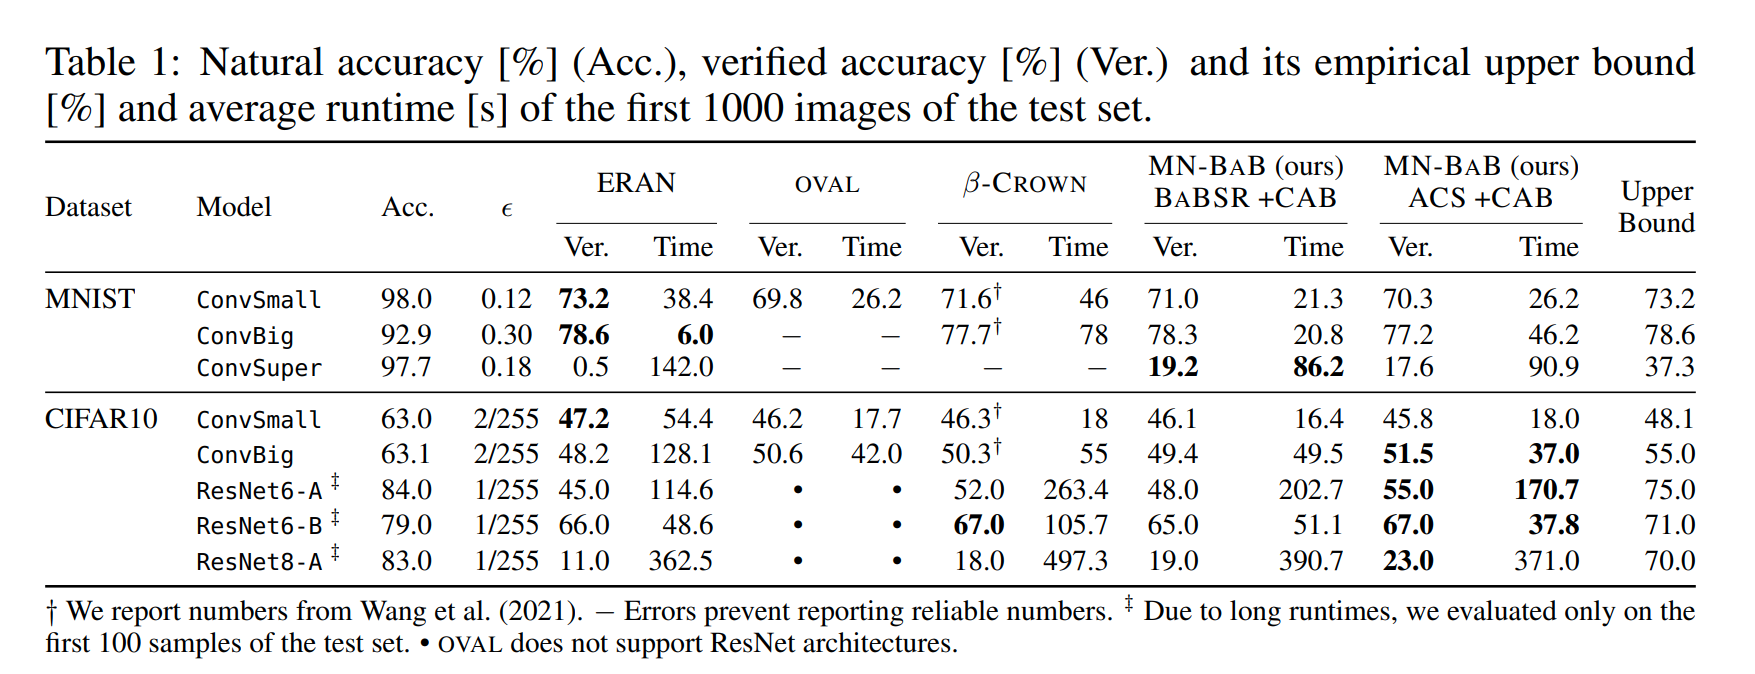
\includegraphics[scale=0.32]{ToMNBAB.png}
\end{figure}



However, their paper did not show those network we focus on. So we run MnBAB on several networks that we considered on our device. The comparison is as follows:



\subsubsection*{PRIMA} 

PRIMA is one of ERAN's major verifier. Its authors have shown its performance in their paper.

Basically, PRIMA is slightly less accuracy and slower than $\alpha,\beta$-Crown for several networks we considered. Here, we directly use the tables from $\alpha,\beta$-Crown's paper:

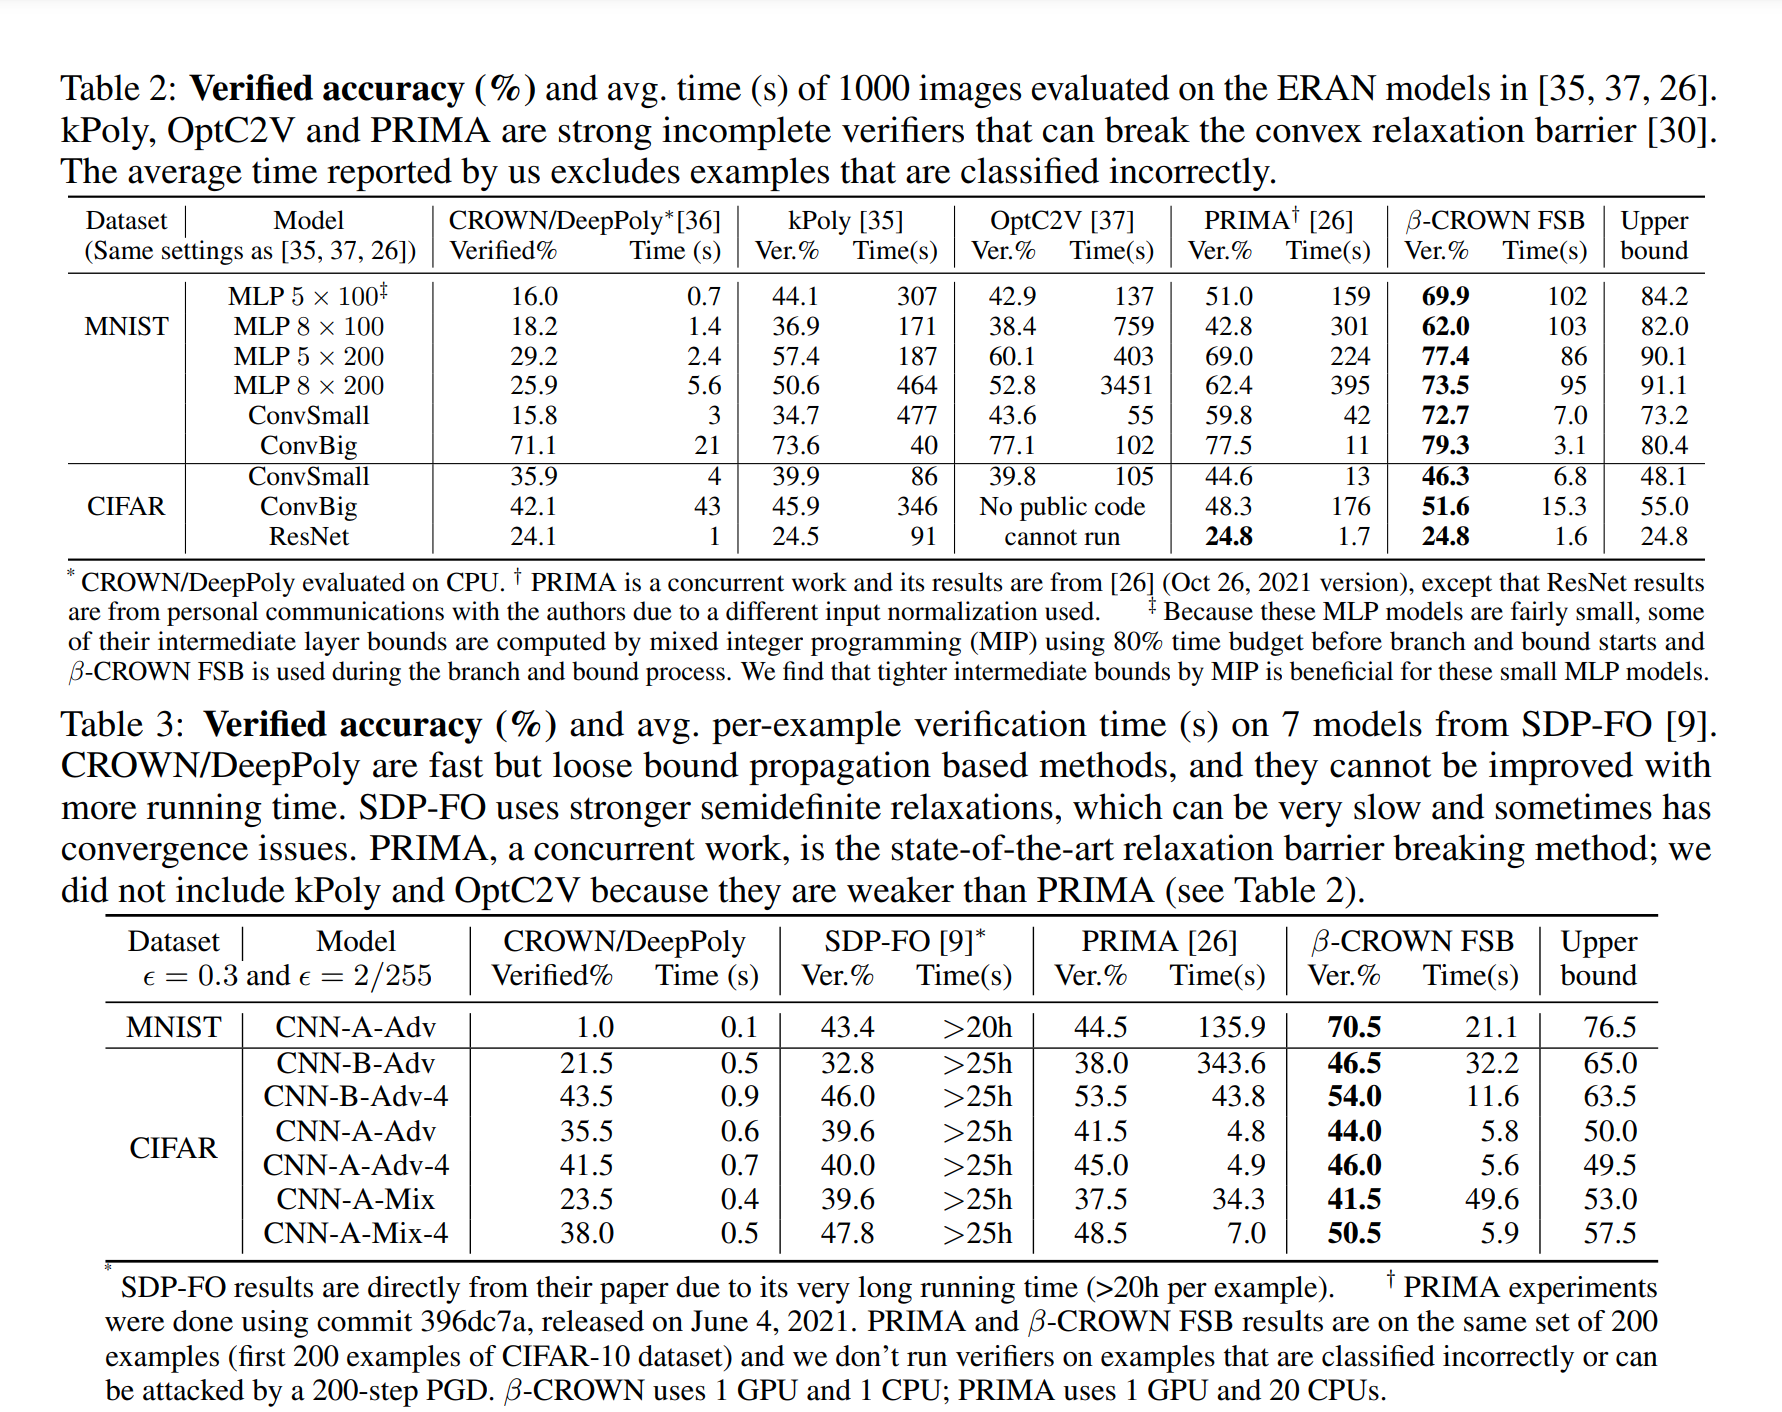
\includegraphics[scale=0.32]{Cronw_PRIMA.png}

\subsubsection*{NNenum} 

We meet some trouble when running CIFAR-CNN-B-Adv and MNIST-6$\times$500.

%As a first step to prove Theorems \ref{th1} and \ref{th2}, 
%we will relax the compensating pairs notion to allows pairs of paths having nodes in common.
%Such a pair is called a {\em weak compensating pair}.
%We will then in a second step prove Theorems \ref{th1} and \ref{th2} for the full definition of compensating pairs of paths.
%
%Let $\cal B$ be a neighbourhood of an input.
%For convenience,
%when the neighbourhood $\cal B$ is clear, 
%we will write $\max(n)$ to denote $\max_{\vx \in \cal B}(\Val_{\vx}(n))$, and $\min(n)$ to denote $\min_{\vx \in \cal B}(\Val_{\vx}(n))$.
%Notice that if $\Val_{\vx}(b)$ is maximal (resp. minimal), 
%then $\Val_{\boldsymbol{x}}(\hat{b})$ also gets maximal (resp. minimal), for $\hat{b}=\texttt{ReLU}(b)$. 
%
%
%We fix a target node $z$.
%We now define the partial influence sign function $S^z$, denoted $S$ when $z$ is clear from the context:
%
%\begin{definition}
%	\label{sign_of_nodes}
%	We define the partial influence sign function $S$ on node $n$: 	
%	\begin{enumerate}
%		\item $S(n)=0$ if all path from $n$ to $z$ have weight $0$; 
%		\item $S(n)=1$ if all path from $n$ to $z$ have non-negative weight, and at least one path has a positive weight; 
%		\item $S(n)=-1$ if all path from $n$ to $z$ have non-positive weight, and at least one path has a negative weight. 
%	\end{enumerate}
%\end{definition}
%
%In general, $S$ may not be defined on every node 
%(e.g. if there is a negative and a positive path from $a$ to $c$). 
%However, if there is no compensating pair of paths, 
%$S$ is defined on all nodes: any node fulfills one of the above cases (1),(2),(3).
%
%For instance for any 3 layer DNN: for an input node $a_i$:
%\begin{enumerate}
%	\item  $S(a_i)=0$ if 
%	for all $b_j, W_{a_i b_j}\cdot W_{b_j c} = 0$
%	
%	
%	\item  $S(a_i)=1$ if for all $b_j, W_{a_i b_j}\cdot W_{b_j c} \geq 0$ and there exists 
%	$j, W_{a_i b_j}\cdot W_{b_j c} > 0$
%	
%	\item $S(a_i)=-1$ if for all $b_j\ W_{a_i b_j}\cdot W_{b_j c} \leq 0$ and there exists 
%	$j, W_{a_i b_j}\cdot W_{b_j c} < 0$ 
%\end{enumerate}
%
%For $b_j$ in the hidden layer, we have $S(b_j)=1,-1,0$ if $W_{b_j c}$ is positive, negative, or 0 respectively. Finally, for the output node $z$, we define $S(z)=1$.
%
%
%
%
%
%\section{Proof of Theorem \ref{th1}}	
%
%
%Assume that there is no (weakly) compensating pair of paths.
%
%
%\begin{lemma}
%	\label{lemma1}
%	Let $L,L'$ be consecutive layers of a DNN without compensation, 
%	$m\in L$ and $n\in L'$. If $W_{m n} \neq 0$ and $S(n) \neq 0$, then 
%	$S(m)=S(n)\mathrm{Sign}(W_{n m})$.
%\end{lemma}
%
%\begin{proof}
%	If $S(n) \neq 0$, then there is a path $\pi$ from $n$ to the output node $z$ with a nonzero weight of the same influence sign as $S(n)$. 
%	So there is a non zero path from $m$ to $z$: $(m n) \pi$, whose influence sign is 
%	$S(n)\mathrm{Sign}(W_{n m})$. As there is no compensation, $S(m)=S(n)\mathrm{Sign}(W_{n m})$.
%	\hfill $\square$
%\end{proof}
%
%
%%For a node $n$, we use $n_s$ to denote $S(n)\cdot n$. 
%%Notice that for $S(n)=1$, $n_s$ gets maximal value whenever $n$ gets maximal value; 
%%while for $S(n)=-1$, $n_s$ gets maximal value whenever $n$ gets minimal value (and vice versa). For $S(n)=0$, $n_s=0$ and thus always reach his minimal and maximal.
%
%Using the concept of influence sign, we introduce input vectors $\vx^{*}, \vx^{\sharp}$: 
%
%\begin{definition}
%We define the following two input vectors $\vx^{*}, \vx^{\sharp}$ in $\cal B$: 
%	\begin{itemize}
%		\item $\vx^{*}$ is the input vector defined in the following way:
%		\begin {itemize}
%		 \item $x^*_{a_i}=\max(a_i)$ if $S(a_i)\in \{0,1\}$, and
%          \item $x^*_{a_i}=\min(a_i)$ otherwise, that is when $S(a_i)=-1$.
%	\end{itemize}
%		
%		\item $\vx^{\sharp}$ is the input vector defined in the following way:
%		\begin{itemize}
%			\item $x^{\sharp}_{a_i}=\min(a_i)$ if $S(a_i)\in \{0,1\}$, and
%			\item $x^{\sharp}_{a_i}=\max(a_i)$ otherwise, that is when $S(a_i)=-1$.
%		\end{itemize}
%	\end{itemize}
%\end{definition}
%
%{Notice that above definitions only involve weights, and do not use bias. As demonstrated by the following lemmas and proofs, our discussion is independent of bias, regardless of whether the bias values are very large or very small.}
%
%We can then prove the following key lemma for Theorem \ref{th1}.
%
%\begin{lemma}
%	\label{lem:key1}
%	\label{lemma2}
%For all $n$ with $S(n)=1$, we have $\val_{\vx^*}(n) = \max(n)$
%and $\val_{\vx^{\sharp}}(n) = \min(n)$.
%For all $n$ with $S(n)=-1$, we have $\val_{\vx^*}(n) = \min(n)$
%and $\val_{\vx^{\sharp}}(n) = \max(n)$. Further, for $L,L'$ two consecutive layers and $n$ on layer $L'$:
%$$\max(n)=\sum_{m \in L, W_{mn}>0}W_{mn} \max(\hat{m}) + \sum_{m \in L, W_{mn}<0}W_{mn} \min(\hat{m}) + bias_n$$
%$$\min(n)=\sum_{m \in L, W_{mn}>0}W_{mn} \min(\hat{m}) + \sum_{m \in L, W_{mn}<0}W_{mn} \max(\hat{m}) + bias_n$$
%
%\end{lemma}
%
%\begin{proof}
%	We prove this lemma by induction on layers. For input layer, this is true by definition. Suppose this lemma is true up to layer $L_i$, we need to show this for layer $L_{i+1}$. Let $n$ be a node in layer $L_{i+1}$, then by definition, we have the following equation: \begin{align*}
%		\val_{\vx}(n) = \sum_{m\in L}W_{m n}\val_{\vx}(\hat{m})) + bias_n.
%	\end{align*}
%	
%	By induction hypothesis, when input vector is $\vx^{*}$, for every $m$, if $S(m)=1$, then $\Val_{\vx^*}(\hat{m})=\max(\hat{m})$ and if $S(\hat{m})=-1$, then $\Val_{\vx^*}(\hat{m})=\min(\hat{m})$. Assume that $S(n)=1$. By applying Lemma \ref{lemma1} and the induction hypothesis:
%	\begin{align*}
%		\val_{\vx^*}(n) = \sum_{m \in L_i, W_{mn}>0}W_{mn} \max(\hat{m}) + \sum_{m \in L_i, W_{mn}<0}W_{mn} \min(\hat{m}) + bias_n\\
%	\end{align*}
%	
%
%
%	Further, we have the following inequality:
%	\begin{align*}
%		\max(n)\leq & \sum_{m \in L_i, W_{mn }>0}W_{mn} \max(\hat{m}) + \sum_{m \in L_i, W_{mn}<0}W_{mn} \min(\hat{m}) + bias_n\\
%		\leq & \val_{\vx^*}(n)
%	\end{align*}
%	
%	%If $S(m)=1$, then by Lemma \ref{lemma1}, $W_{mn}>0$; if $S(m)=-1$, then $W_{mn}<0$; if $S(m)=0$, then $W_{mn}=0$.
%	
%	By definition of $\max$, we have $\val_{\vx^*}(n) \leq \max(n)$.
%	Combining the 2 formulas, we obtain $\max(n)=\Val_{\vx^*}(n)$. 
%	
%	We prove similarly that $\min(n)=\Val_{\vx^\sharp}(n)$,
%	and the case $S(n)=-1$. This concludes the induction. 
%\end{proof}
%
%{ As we mentioned earlier, this proof does not have any requirements on the bias.}
%
%\iffalse
%	As direct corollary of Lemma \ref{lem:key1}, we obtain:
%	
%	\begin{corollary}
%		\label{cor1}
%		$$\max(c)=\sum_{b \in L, W_{bc}>0}W_{bc} \max(\hat{b}) + \sum_{b \in L, W_{bc}<0}W_{bc} \min(\hat{b}) + bias_c$$
%		$$\min(c)=\sum_{b \in L, W_{bc}>0}W_{bc} \min(\hat{b}) + \sum_{b \in L, W_{bc}<0}W_{bc} \max(\hat{b}) + bias_c$$
%	\end{corollary}
%	
%\fi
%	
%	%Notice that for all $x$, for either $S(c)=1$ or $S(c)=-1$, these two bounds are found in Lemma \ref{lemma2},
%	%from configuration $\boldsymbol{x}^*$ and $\boldsymbol{x}^\sharp$.
%	
%	
%	
%	
%	
%	\subsubsection*{Bounds generated by Value Abstraction}
%
%	\smallskip
%	
%	Let $[\alpha_n,\beta_n]$ be the bounds generated by the Box abstraction.
%	We show that these bounds are exact when there is no (weak) compensating pairs of paths, i.e. for all node $n$ of the DNN, we have $\alpha_n=\min(n)$ and $\beta_n=\max(n)$.
%
%\begin{proof}
%	 We show that inductively. The initialization is obvious as Box Abstraction is always exact for the first layer.
%
%	Let $n$ be node of the DNN. We set the target $z=n$ and consider the influence sign function $S^z=S^n=S$ corresponding to that node. By definition, $S(n)=1$. 
%	
%	The Box abstraction computes its upper bound using:
%	$$\beta_n= \sum_{W_{mn}>0} W_{mn} \beta_{\hat{m}} + \sum_{W_{mn}<0} W_{mn} \alpha_{\hat{m}} + bias_n$$
%
%	By induction hypothesis, we have 
%		$\beta_{\hat{m}}=\max(\hat{m})$ and
%		$\alpha_{\hat{m}}=\min(\hat{m})$, thus 
%		applying the second part of Lemma \ref{lem:key1}, we obtain
%		$\beta_n=\max(n)$.
%		
%		Similarly, we obtain $\alpha_n=\min(n)$.
%		
%		Consider now $\alpha_{\hat{n}},\beta_{\hat{n}}$.
%		If $\alpha \leq 0$ then $\alpha_{\hat{n}}=0=\max(\hat{n})$.
%		Otherwise, $\alpha_{\hat{n}}=\alpha_n=\max(\hat{n})$.
%		In both case it is exact.
%
%		Similarly, if $\beta_n=\max(n)<0$, 
%		then $\beta_{\hat{n}}=\max(\hat{n})=0$, 
%		and otherwise 
%		$\beta_{\hat{n}}=\max(\hat{n})=\beta_n=\max(n)$.
%		
%		Hence we have equality pre and post activation function.
%			\end{proof}
%	
%
%
%This shows the statement of Theorem 1 with the weaker statement that there is no weak compensating pairs of paths.
%
%	
%	
%	\subsubsection*{From weak to normal}
%	
%	\begin{lemma}
%		If a DNN has no compensating pair, then it also does not have weak compensating pair from an input node to the output node.
%	\end{lemma}
%	
%	\begin{proof}
%		By contradiction, if there is a weak compensating pair of two paths, $\rho_1,\rho_2$, 
%		then consider the common nodes by increasing layer $n_1 \cdots n_k$ in $\rho_1,\rho_2$ (including the initial and final nodes).
%		Assume that there is no compensating pair.
%		It means that all the segment of $\rho_1,\rho_2$ from $n_i$ to $n_{i+1}$ have the same influence sign (they have no nodes in common but the initial and final nodes).
%		Hence $\rho_1$ and $\rho_2$ have the same influence sign, a contradiction with $\rho_1,\rho_2$ being a weakly compensating pair. 
%	\end{proof}
%	
%	This finishes the proof of Theorem \ref{th1}.
%	
%	
%
%
%
%
%
%
%\newpage
%
%
%
%
%
%	
%
%
%
%
%
%			
%\section{Proof of Theorem \ref{th2}}
%			
%			In this section, we will prove theorem \ref{th2}. We first prove the following weaker theorem:
%			
%			\begin{theorem} \label{thm:2}	
%				Suppose $\mathcal{D}$ is a DNN with a unique output node $z$.
%				Let $X$ be the set of nodes $n$ such that there is a weak compensating path 
%				passing by $n$ (except its source and target nodes).
%				Then $\MILP_X$ computes the exact bounds $[\alpha,\beta]$ for $z$,
%				i.e. $\alpha=\min(z)$ and $\beta=\max(z)$.
%			\end{theorem}
%			
%			
%			\subsection{Proof of Theorem \ref{thm:2}}
%			
%			\begin{definition}
%				We define a partition of the set $A$ of input nodes as $A_{zero} \sqcup A_{pure}\sqcup A_{open}$, with:  
%				\begin{itemize}
%					\item $A_{zero}= \{a \mid \forall \text{ path $\rho$ from $a$ to } z, weight(\pi)=0\}$.
%	
%					\item $a_k \in A_{pure}$  if $a \notin A_{zero}$ and either
%					\begin{enumerate}
%						\item every path from $a_k$ to $z$ has weight $\geq 0$, or
%						\item every path from $a_k$ to $z$ has weight $\leq 0$. 
%						
%					\end{enumerate}
%					Hence, $a_k$ is not a source of a weak compensating pair. We denote 
%					$A_{pure}$ by $I$ for short.
%					\item $a_k \in A_{open}$ iff $a_k \notin A_{pure} \sqcup A_{zero}$, that is there exists two paths $\rho,\rho'$ from $a_k$, one with positive and one with negative weight. 	We denote $A_{open}$ by $J$ for short.
%				\end{itemize}
%			\end{definition} 
%			
%
%			
%			\begin{lemma} \label{lem:open_node_2}
%				A node $b$ in a hidden layer will not be on a weak compensating path if and only if one of the following happens:
%				\begin{enumerate}
%					\item Any path from $b$ to the output node $z$ has a weight $0$, and we use $weight({bz})=0$ to denote this case, or
%					\item For every input node $a_j\in J$, every path from $a_j$ to $b$ has a weight of $0$. We use $weight({a_jb})=0$ to denote this case.
%				\end{enumerate}
%				
%			\end{lemma}
%			
%			We denote $B_{zero}$ the set of nodes $b$ that case 1 holds, and denote $B_{pure}$ the set of nodes $b$ such that case 2 holds but case 1 does not hold.
%			We denote $B_{open}$ the set of all nodes $b$ in a weak compensating path (remaining cases).
%			
%		{ 	Similarly, above definitions $A_{zero},A_{open}, A_{pure}$ and $B_{zero},B_{open},B_{pure}$ do not consider bias, and any kind of bias will not affect our theorem.}
%		
%		\begin{figure}[h]
%			\centering
%			\begin{tikzpicture}[>=stealth, node distance=2cm]
%				% Input nodes (two types)
%				\node[circle, draw, minimum size=0.5cm] (input1) at (-1,0) {$a_0$};
%				\node[circle, draw, minimum size=0.5cm] (input2) at (-2,0) {$a_1$};
%				\node[circle, draw, minimum size=0.5cm] (input3) at (-4,0) {$a_2$};
%				
%				\node[circle, draw, minimum size=0.5cm] (input4) at (-5,0) {$a_3$};
%				\node[circle, draw, minimum size=0.5cm] (input5) at (-7,0) {$a_4$};
%				\node[circle, draw, minimum size=0.5cm] (input6) at (-8,0) {$a_5$};
%				
%				\draw[draw=black, dashed] (-1.5,0) ellipse (1.35 and 0.75);
%				\node[below] at (-1.5,-0.75) {$A_{zero}$};
%				
%				\draw[draw=black, dashed] (-2,2) ellipse (0.75 and 0.75);
%				\node[right] at (-1,2) {$B_{zero}$};
%				
%				% Hidden layer nodes
%				
%				\node[circle, draw, minimum size=0.5cm, fill=blue!20] (hidden1) at (-2,2) {$n_0$};
%				
%				\node[circle, draw, minimum size=0.5cm, fill=blue!20] (hidden2) at (-4,2) {$n_1$};
%				\node[circle, draw, minimum size=0.5cm, fill=blue!20] (hidden3) at (-5,2) {$n_2$};
%				
%				\node[circle, draw, minimum size=0.5cm, fill=blue!20] (hidden4) at (-7,2) {$n_3$};
%				\node[circle, draw, minimum size=0.5cm, fill=blue!20] (hidden5) at (-8,2) {$n_4$};
%				
%				
%				
%				\draw[draw=black, dashed] (-4.5,0) ellipse (1.35 and 0.75);
%				\node[below] at (-4.5,-0.75) {$A_{pure}$};
%				
%				
%				\draw[draw=black, dashed] (-7.5,0) ellipse (1.35 and 0.75);
%				\node[below] at (-7.5,-0.75) {$A_{open}$};
%				
%				
%				
%				\draw[draw=black, dashed] (-4.5,2) ellipse (1.35 and 0.75);
%				\node[left] at (-3.5,3) {$B_{pure}$};
%				
%				
%				\draw[draw=black, dashed] (-7.5,2) ellipse (1.35 and 0.75);
%				\node[left] at (-8.5,1.5) {$B_{open}$};
%				
%				
%				
%				% Output node
%				\node[circle, draw, minimum size=0.8cm, fill=red!20] (output) at (-5,4) {$z$};
%				
%				
%				% connections
%				
%				\draw[->] (input1) -- (hidden1);
%				
%				\draw[->] (input3) -- (hidden5);
%				
%				\draw[->] (input4) -- (hidden4);
%				
%				
%				%		% Connect input to hidden layer
%				\foreach \i in {3,4} {
%					\foreach \h in {3,2} {
%						\draw[line width=1.5pt, ->] (input\i) -- (hidden\h);
%					}
%				}
%				
%				
%				\foreach \i in {5,6} {
%					\foreach \h in {4,5} {
%						\draw[->] (input\i) -- (hidden\h);
%					}
%				}
%				%		
%				% Connect hidden layer to output
%				\foreach \h in {2,3} {
%					\draw[line width=1pt,->] (hidden\h) -- (output);
%				}
%				
%				\foreach \h in {4,5} {
%					\draw[->] (hidden\h) -- (output);
%				}
%				
%				%\		% Input label
%				\node[left=0.7cm of input6] {Input Layer};
%				
%				% Hidden label
%				\node[left=0.7cm of hidden5] {Hidden Layer};
%				
%				% Output label
%				\node[left=0.5cm of output] {Output Layer};
%			\end{tikzpicture}
%			\caption{Definitions in the proof of Theorem \ref{th2}}
%			\label{fig:neural_network_types_simplified}
%		\end{figure}
%			
%			\begin{proof}
%				First, we show that if one of case 1, 2 happens, then $b$ will not be in a weak compensating pair. If 1), it is obvious. For 2, we reason by contradiction: assume there is a pair of weak compensating paths 	$(\pi,\pi')$ starting with $a$, with $b$ in $\pi$ and weight$(\pi) > 0$. It means that $a \in J$. This is a contradiction as 2) $weight({a_j,b})=0$ implies weight$(\pi)=0$.
%				
%				Second, we show that if neither 1 nor 2 hold, then $b$ will be in a weak compensating path.
%				Because 2) does not hold, there exists $a_j \in J$ with $weight({a_j,b}) \neq 0$, say $>0$.
%				Because 1) does not hold, $weight({b,z}) \neq 0$, say $>0$.
%				Now, by definition of $J$, there is a pair of weak compensating paths $\pi,\pi'$ 
%				from $a_j$ to $z$, say with $\pi'$ with weight $<0$.
%				Then two paths $(a_j,b,z)$ and $\pi'$ also form a weak compensating pair.
%			\end{proof}
%			
%						
%			
%			\begin{lemma}\label{lem:subnetwork}
%				$I \cup B_{pure} $ forms a sub-network, denoted $D_I$. That is, 
%				for $n \in B_{pure}$, for every path $\rho$ from $m$ to $n$
%				either $m \in B_{pure}\cup I$ or $weight(\rho)=0$.
%				Further, in $D_I$, there is no (weakly) compensating pair.
%			\end{lemma}
%
%			
%
%			
%			\begin{proof}
%				This is simply because for a node $c\in B_{pure}$ in a hidden layer or the output layer, for a node $b$ in one layer before, if $b\notin B_{pure}\cup I$, then:
%				
%				1. if $b\in J$, by definition, $W_{bc}=0$.
%				
%				2. if $b\in B_{open}$, then $W_{bc}=0$; otherwise there exists $<a_j,b,c>$ a path from $a_j\in J$ to $c$ with a nonzero value, a contradiction.
%				
%				3. if $b\in B_{zero}$, then $W_{bc}=0$; otherwise there exists $<b,c,z>$ a path from $b$ to $z$ the output node with a nonzero value, a contradiction. 
%			\end{proof}
%			
%			
%			
%			For an input $\vx$ and a subset $S$ of input nodes, we denote by 
%			$\boldsymbol{x}_S$ to refer the input vector $\langle x_{a_k}\rangle_{a_k\in S}$. We use $\boldsymbol{x}_I\oplus \boldsymbol{x}_J = \boldsymbol{x}$ and 
%			$\Val_{\boldsymbol{x}_I,\boldsymbol{x}_J} (z)=\Val_{\boldsymbol{x}}(z)$. 
%			
%			
%			Invoking Lemma \ref{lem:subnetwork}, we can apply Theorem 1 on $D_I$, and obtain two input vectors $\boldsymbol{x}_I^*,\boldsymbol{x}_I^{\sharp}$ on $I$
%			minimizing and maximizing all the nodes in $D_I$.
%
%			\smallskip
%
%		
%			Recall the influence sign function of nodes from Definition \ref{sign_of_nodes}. 
%			Because weakly compensating paths are allowed, the influence sign function is no longer defined on all nodes. $S$ is defined for all nodes from which there is no weakly compensating pairs of paths to $z$. In particular, $S$ is defined on all nodes of $I$.
%
%			\begin{lemma}\label{lem:sign}
%				Let $m,n$ be two nodes, such that $S$ is defined on $m$ and there is a path $\rho$ with non zero weight to a node $n$. Then $S$ is defined on $n$
%				 (there is no compensating pair of paths from $n$ to $z$).
%				Further, $S(n)= Sign(weight(\rho)) S(m)$.
%			\end{lemma}
%			
%			\begin{proof}
%				By contradiction, assume that there exists two paths $\rho_1,\rho_2$ from 
%				$n$ to $z$ with (strictly) different influence signs. The pair $\langle a_i,n\rangle \cdot \rho_1$ and $\langle a_i,n\rangle \cdot \rho_2$ is compensating, a contradiction with $a_i\in I$. 
%			\end{proof}
%
%			Hence, for all node $n$, either $S$ is defined on $n$, or 
%			$n$ depends only upon input nodes in $J$.
%			Let us call $D_J$ the set of such nodes which only depends upon nodes in $J$.
%			$D_J$ forms a sub-network.
%			$D_J$ contains the set of all nodes from which there is a weakly compensating pair of paths to $z$.
%			By definition, for any $b\in D_J$, either $b\in B_{open}$, or $b$ is a constant node: any path from any input node must have zero weight to it.
%			For a node $b$ for which $S$ is undefined, $b$ thus only depends on $J$; so, if $\boldsymbol{x}_J$ is fixed, then the value of $b$ will be fixed.
%			Notice that $D_I \sqcup D_J$ does not cover the DNN entirely in general.
%			
%			
%			
%			\begin{lemma} \label{lem:reach_max_2}
%				Let $n$ be a node on which $S$ is defined. If $S(n)=1$,
%				for any valuation $\boldsymbol{x}^0_J$,	we have: 
%				$$\max_{\boldsymbol{x}_I} (\Val_{\boldsymbol{x}_I,\boldsymbol{x}^0_J}(b)) =  \Val_{\boldsymbol{x}_I^*,\boldsymbol{x}^0_J}(b).$$
%				
%				$$\min_{\boldsymbol{x}_I} (\Val_{\boldsymbol{x}_I,\boldsymbol{x}^0_J}(b)) =  \Val_{\boldsymbol{x}_I^{\sharp},\boldsymbol{x}^0_J}(b).$$
%				
%				
%				If $S(b)=-1$, 
%				$$\max_{\boldsymbol{x}_I} (\Val_{\boldsymbol{x}_I,\boldsymbol{x}^0_J}(b)) =  \Val_{\boldsymbol{x}_I^{\sharp},\boldsymbol{x}^0_J}(b).$$
%				
%				$$\min_{\boldsymbol{x}_I} (\Val_{\boldsymbol{x}_I,\boldsymbol{x}^0_J}(b)) =  \Val_{\boldsymbol{x}_I^{*},\boldsymbol{x}^0_J}(b).$$	
%			\end{lemma}
%			
%			\begin{proof}	
%				Fix an input vector $\boldsymbol{x}^0_J$.
%				This also fixes the values in $D_J$.
%				Consider the DNN $D'$ with input nodes $a_i\in I$, where all the 
%				edges from $m \in D_J$ to $n$ are replaced by a bias (equals to the weight of the edge times the fix value $\val_{\boldsymbol{x}^0_J}(m)$) for $n$ (we sum all these bias for a neuron $n$).
%				We denote $\val'$ values of nodes in this DNN $D'$.
%				 
%				We have $\Val_{\boldsymbol{x}_I,\boldsymbol{x}^0_J}(z) = \val'_{\boldsymbol{x}_I}(z)$.
%				In the simplified $D'$, there is no weakly compensating path to $z$ because 
%				$D_J$ contains all the source of weakly compensating path to $z$.
%				Therefore we can apply Lemma \ref{lem:key1} to get that 
%				$\val'_{x_I}(z)$ reaches its maximal value for $\boldsymbol{x}_I=\boldsymbol{x}_I^*$, and conclude by using $\Val_{\boldsymbol{x}_I,\boldsymbol{x}^0_J}(z) = \val'_{\boldsymbol{x}_I}(z)$. The case for min is similar. 
%			\end{proof}
%			
%			From Lemma \ref{lem:reach_max_2}, we immediatly obtain the following corollary:
%
%			\begin{corollary}
%				\label{corr:main}
%			For a node $b$ with $S(b)=1$:
%		
%			$$\max(b)=\max_{\vx_J} \val_{\vx^{\star}_I,\vx_J}(b)$$
%			$$\min(b)=\min_{\vx_J} \val_{\vx^{\sharp}_I,\vx_J}(b)$$
%			and for $S(b)=-1$:
%	
%			$$\max(b)=\max_{\vx_J} \val_{\vx^{\sharp}_I,\vx_J}(b)$$
%			$$\min(b)=\min_{\vx_J} \val_{\vx^{\star}_I,\vx_J}(b)$$
%			\end{corollary}
%			
%	
%			
%
%
%			%\subsection{$\MILP_X$ is accurate}
%			
%			
%
%
%
%
%
%			%We want to show that $\beta= \max(z)$. 
%			%As the MILP abstraction is a sound over-approximation, it suffices to show that %$\beta\leq \max (z)$.
%			%The case for $\alpha$ is similar.
%			
%			
%			%\begin{lemma}
%			%	Both $D_I$ and $D_J$ are accurate in the sense that for any $b$ in $D_I$ or %$D_J$, $\UB(b)=\max(b)$ and $\LB(b)=\min(b)$.
%			%\end{lemma}
%			
%			%\begin{proof}
%			%	For $D_I$, it is because of no compensating as proved in the first section. %For $D_J$, it is because all nodes are either opened or constants. 
%			%\end{proof}
%			
%			
%			%\begin{definition} Assume $\boldsymbol{x}^0_I\oplus \boldsymbol{x}^0_J$ is a input vector, and $b$ is node in hidden layers or output layer.
%			%
%			%	1. For a given vector $\boldsymbol{x}$ , $\B_{\boldsymbol{x}^0_I, \boldsymbol{x}^0_J, \boldsymbol{x}}(b)$ is the value of $b$ in the MILP model for values $\boldsymbol{x}^0_I, \boldsymbol{x}^0_J, \boldsymbol{x}$.
%			%\end{definition}
%\iffalse			
%			For input vectors $\boldsymbol{x}^0_I,\boldsymbol{x}^0_J$, let $\UB_{\boldsymbol{x}^0_I,\boldsymbol{x}^0_J}(b)$ be the upper bound in the above fixed formulation and framework while the input $\boldsymbol{x}^0_I,\boldsymbol{x}^0_J$ is fixed: that is, besides the constraints in above MILP models, we add new constraints $\boldsymbol{x}_I,\boldsymbol{x}_J=\boldsymbol{x}^0_I,\boldsymbol{x}^0_J$. We  define $\LB_{\boldsymbol{x}^0_I,\boldsymbol{x}^0_J}(b)$ similarly for $\LB$ lower bound. For them, we have the following lemma:
%			
%			\begin{lemma} In an MILP formulation, for a node $c$ in a hidden layer or output layer:
%				
%				1. $\UB(b)=\max_{\boldsymbol{x}^0_I,\boldsymbol{x}^0_J}\UB_{\boldsymbol{x}^0_I,\boldsymbol{x}^0_J}(c)$. 
%				
%				2. $\LB(b)=\min_{\boldsymbol{x}^0_I,\boldsymbol{x}^0_J}\LB_{\boldsymbol{x}^0_I,\boldsymbol{x}^0_J}(c)$. 
%			\end{lemma}
%			
%			\begin{proof}
%				This is by the definition of MILP formulation and $\UB_{\boldsymbol{x}^0_I,\boldsymbol{x}^0_J}, \LB_{\boldsymbol{x}^0_I,\boldsymbol{x}^0_J}$. 
%			\end{proof}
%			
%	
%			
%			
%		%We will prove this by induction on layers from the first hidden layer to the output layer. More specifically, we will prove the following lemmas:
%			
%	
%
%		\begin{lemma} \label{lem:main}
%				For any node $c$ in a hidden layer or the output layer, if $c\notin B_{zero}$, then:		\begin{enumerate}
%					\item for any fixed $\boldsymbol{x}^0_J$, when  $\boldsymbol{x}_I=\boldsymbol{x}^*_I$, the value for $c$ in the MILP model is a fixed number, and naturally $\UB_{\boldsymbol{x}^*_I,\boldsymbol{x}^0_J}(c)=\LB_{\boldsymbol{x}^*_I,\boldsymbol{x}^0_J}(c)$. The same is true for $\boldsymbol{x}^\sharp_I$.
%					
%					\item for any fixed $\boldsymbol{x}^0_J$, if $S(c)=1$, then $$\max_{\boldsymbol{x}_I} \UB_{\boldsymbol{x}_I,\boldsymbol{x}^0_J}(c)=\UB_{\boldsymbol{x}^*_I,\boldsymbol{x}^0_J}(c)= \Val_{\boldsymbol{x}^*_I,\boldsymbol{x}^0_J}(c) = \max_{\boldsymbol{x}_I} \Val_{\boldsymbol{x}_I,\boldsymbol{x}^0_J}(c).$$ The similar for $S(c)=-1$, $\langle \LB,\min\rangle$, $x^\sharp_I$: we can change two of them at the same time.
%					
%					\item Therefore, $\UB(c)=\max(c)$ and $\LB(c)=\min(c)$.
%				\end{enumerate}
%				
%				
%				
%			\end{lemma}
%			
%
%
%			\begin{proof}
%				We prove this lemma by induction on layers. For first hidden layer $L_1$, it is obvious. Suppose we have proved part 1,2,3 up to layer $L_i$, then for layer $L_{i+1}$, suppose $c$ is a node in this layer. 
%				
%				(1)	If $S(c)$ is undefined, then by previous discussion, $c$ is in a sub-network from $J$ with all nodes opened; and if $\boldsymbol{x}_J=\boldsymbol{x}_J^0$ is fixed, then in the MILP model, the value for $c$ is also fixed. 
%				
%				If $S(c)$ is defined, then consider all $b$ such that $W_{bc}\neq 0$. First, $b$ cannot in $B_{zero}$; so by induction hypothesis, the value of $b$ is fixed under $\boldsymbol{x}^*_I,\boldsymbol{x}^0_J$ in MILP model. 
%				
%				
%				
%				If $b\in B_{open}$, the term is $W_{bc}\ReLU(b)$. We know then by induction hypothesis, the value for $b$ in MILP is a fixed value. Then the term $W_{bc}\ReLU(b)$ is also a fixed number.  
%				
%				If $b\in B_{pure}$, the term is $W_{bc}\mathrm{AppB}(b)$ ($\mathrm{AppB}$ is the LP approximation domain of $\ReLU$) and either $S(b)$ is undefined and $b$ is a constant in the network and so is in the MILP model (trivial case), or $S(b)$ is defined. 
%				
%				Then by induction hypothesis for all 1, 2 and 3 parts,  the value of $b$ in the model is fixed (part 1), and it is equal to $\max_{\boldsymbol{x}_I} \Val_{\boldsymbol{x}_I,\boldsymbol{x}^0_J}(c)$ or $\min_{\boldsymbol{x}_I} \Val_{\boldsymbol{x}_I,\boldsymbol{x}^0_J}(c)$ (by part 2, depending on $S(b)$). Since $b$ only depends on $I$, this value also equal to $\max_{\boldsymbol{x}_I} \Val_{\boldsymbol{x}_I}(c)$ or $\min_{\boldsymbol{x}_I} \Val_{\boldsymbol{x}_I}(c)$, and by induction hypothesis on part 3, equal to $\UB(b)$ or $\LB(b)$. For either of them, $\mathrm{AppB}(b)$ will be fixed value. Hence, in this case, the term $W_{bc}\mathrm{AppB}(b)$ is also a fixed number.
%				
%				Therefore, in the MILP model, $c$ is a sum of terms that are all fixed numbers. Hence $c$ is a fixed number.
%				
%				(2) If $S(c)=1$, then we have the following:	\begin{align*}
%					\mathrm{UB}_{\boldsymbol{x}^0_J,\boldsymbol{x}^0_I}(c) \leq constant + \sum_{b\in B_{open}\cap l_i} W_{bc}\ReLU(\B_{\boldsymbol{x}^0_I,\boldsymbol{x}^0_J}(b)) + \sum_{b\in B_{pure}\cap l_{i}} W_{bc} \mathrm{AppB}(\B_{\boldsymbol{x}^0_I,\boldsymbol{x}^0_J}(b)),
%				\end{align*}where $\B$ means one of $\UB$ or $\LB$ depending on the influence sign of $W_{bc}$: if $W_{bc}$ is positive, then $\UB$, otherwise $\LB$. Notice that all $b$ displayed are that $S(b)$ defined, because if $S(b)$ undefined, then for fixed $\vx_J$, value of $b$ is fixed and will be put into the constant.
%				
%				Now by induction hypothesis part 2, if $S(b)=1$, then $\UB_{\boldsymbol{x}^*_I,\boldsymbol{x}^0_J}(b)=\max_{\vx_I}\UB_{\boldsymbol{x}^*_I,\boldsymbol{x}^0_J}(b)$; and if $S(b)=-1$, $\LB_{\boldsymbol{x}^*_I,\boldsymbol{x}^0_J}(b)=\min_{\vx_I}\LB_{\boldsymbol{x}^*_I,\boldsymbol{x}^0_J}(b)$. Moreover, since $S(c)=1$, $S(b)$ and $W_{bc}$ have the same influence sign. And both $\ReLU$ and $\mathrm{AppB}$ are non-decreasing functions. Combining all these facts, we have:\begin{align*}
%					\mathrm{UB}_{\boldsymbol{x}^0_J,\boldsymbol{x}^0_I}(c)\leq 
%					&constant + \sum_{b\in B_{open}\cap l_i} W_{bc}\ReLU(\B_{\boldsymbol{x}^*_I,\boldsymbol{x}^0_J}(b)) + \sum_{b\in B_{pure}\cap l_{i}} W_{bc} \mathrm{AppB}(\B_{\boldsymbol{x}^*_I}(b))\\
%					= & \mathrm{UB}_{\boldsymbol{x}^0_J,\boldsymbol{x}^*_I}(c). 
%				\end{align*}  This is the first equal.
%				
%				The second is simply because $\UB_{\boldsymbol{x}^*_I,\boldsymbol{x}^0_J}(c)\geq \Val_{\boldsymbol{x}^*_I,\boldsymbol{x}^0_J}(c)\geq\LB_{\boldsymbol{x}^*_I,\boldsymbol{x}^0_J}(c)$.	The third equal is proved in last subsection, Lemma \ref{lem:reach_max_2}. The case $S(c)=-1$ is similar. This is for part 2.
%				
%				(3) Once we have part 2, we will have that for any fixed $\boldsymbol{x}^0_J$, $$\max_{\boldsymbol{x}_I} \UB_{\boldsymbol{x}_I,\boldsymbol{x}^0_J}(c)= \max_{\boldsymbol{x}_I} \Val_{\boldsymbol{x}_I,\boldsymbol{x}_J}(c).$$ Therefore, $\max_{\boldsymbol{x}_I,\boldsymbol{x}_J} \UB_{\boldsymbol{x}_I,\boldsymbol{x}_J}(c)= \max_{\boldsymbol{x}_I,\boldsymbol{x}_J} \Val_{\boldsymbol{x}_I,\boldsymbol{x}_J}(c)$ and this is to say $\UB(c)=\max(c)$. This is what we want to show, and the same result holds for lower bound and minimal value. This is for part 3. 
%
%			\end{proof}
%
%	\fi
%
%
%
%	We denote by $X=B_{open}$, and consider $\MILP_{X}$.
%	Let $[\alpha,\beta]$ be the bounds computed by $\MILP_{X}$ for the target node $z$. We are now ready to finish the proof of Theorem \ref{thm:2}.
%
%			
%\begin{proof}[Proof of Theorem \ref{thm:2}]
%	We show that $\beta=\max(z)$.
%
%	We fix the input vector $\vx^*_I$ for input $I$.
%	This also fixes the values in $D_I$.
%	Consider the DNN $D'$ with input nodes $J$, where all the 
%	edges from $m \in D_I$ to $n$ are replaced by a bias (equals to the weight of the edge times the fix value $\val_{\boldsymbol{x}^*_I}(m)$) for $n$ (we sum all these bias for a neuron $n$). We denote $\val'$ values of nodes in this DNN $D'$.
%		 
%	We have $\val'_{\boldsymbol{x}_J}(n)=\Val_{\boldsymbol{x}^*_I,\boldsymbol{x}_J}(n)$ 
%	for every node $n$ of $D'$. All the ReLU nodes of $D'$ are in $X$, by definition of $X$.
%Thus $\MILP_X$ will be fully accurate in $D'$. Let $\beta'$ denote its upper bound.
%We have $\beta'=\max_{\vx{_J}} (\val'_{\vx_{J}}(z)) = 
%\Val_{\boldsymbol{x}^*_I,\boldsymbol{x}_J}(n) = \max(z)$ by Corollary \ref{corr:main}.
%Now, in $D$, $\MILP_X$ will use simple LP on $D_I$, which suffices to get the upper bound $\val_{\vx^*_I}(n)=\max(n)$ for all $n$ in $D_I$ and the values will be pushed as bias in $D'$. Therefore, $\beta'=\max(z)$.
%
%We now prove that $\beta=\beta'$, which terminates the proof, as The case for $\alpha=min(z)$ is similar. 
%
%We prove by induction from the input layer to higher layers that the upper bound of node $n$ in $D'$, is greater than or equal to the upper bound in $D$; and similarly for the lower bound. We use  $\Val^{D}_{x_J^0}(n)$ to denote the range of possible values for node $n$ in  model $D$ or $D'$ when $x_J=x_J^0$. 
%This may be a single number or an interval. 
%Denote by $\beta_{x_J^0}(m)$ (resp $\beta'_{x_J^0}(m)$) the upper bound computed by $\MILP_X$ 
%for $m$ in $D$ (resp. $D'$) when the $J$ input is fixed to be ${x_J^0}$.
%We define in the same way  $\alpha_{x_J^0}(m)$ and $\alpha'_{x_J^0}(m)$ for the minimal values.
%
%For any input $x_J=x_J^0$, we prove $\beta'_{x_J^0}(n) \geq \beta_{x_J^0}(n)$ 
%and
%$\alpha'_{x_J^0}(n) \leq \alpha_{x_J^0}(n)$ 
%by induction on $n$:
%
%
%\begin{align*}
%\beta'_{x_J^0}(n) = & {bias}_n+\sum_{m\in B_{pure},W_{mn}>0} W_{mn} \beta'(\hat{m})+\sum_{m\in B_{pure},W_{mn}<0} W_{mn} \alpha'(\hat{m})\\
%+&\sum_{m\notin B_{pure},W_{mn}>0} W_{mn} \beta'_{x_J^0}(\hat{m})+\sum_{m\notin B_{pure},W_{mn}<0} W_{mn} \alpha'_{x_J^0}(\hat{m})\\
%\\
%(\text{by induction})\geq & {bias}_n+\sum_{m\in B_{pure},W_{mn}>0} W_{mn} \beta'(\hat{m})+\sum_{m\in B_{pure},W_{mn}<0} W_{mn} \alpha'(\hat{m})\\
%+&\sum_{m\notin B_{pure},W_{mn}>0} W_{mn} \beta_{x_J^0}(\hat{m})+\sum_{m\notin B_{pure},W_{mn}<0} W_{mn} \alpha_{x_J^0}(\hat{m})\\
%\\
%(\text{Lemma \ref{lem:key1}})= & {bias}_n+\sum_{m\in B_{pure},W_{mn}>0} W_{mn} \beta(\hat{m})+\sum_{m\in B_{pure},W_{mn}<0} W_{mn} \alpha(\hat{m})\\
%+&\sum_{m\notin B_{pure},W_{mn}>0} W_{mn} \beta_{x_J^0}(\hat{m})+\sum_{m\notin B_{pure},W_{mn}<0} W_{mn} \alpha_{x_J^0}(\hat{m})\\
%\geq & \beta_{x_J^0}(n)
%\end{align*} 
%
%The case for $\alpha$ is similar, proving the induction.
%
%Hence, using the $\max$ over ${x_J^0}$, 
%we will have $\max(z) = \beta'\geq \beta \geq \max(z)$, and hence $\beta=\beta'=\max(z)$.\end{proof}
%
%{ In all the statements and proofs above, we do not make any assumptions about bias, and bias will not affect our discussion. }
%
%\subsection{Proof of Theorem \ref{th2}}
%
%
%We now prove Theorem \ref{th2} under the fairly light {\em well-connected hypothesis} (H1) that the DNN is such that for every 2 (not necessarily disjoint) paths $\rho_1,\rho_2$ with non-zero weight with the same source $m$ and the same target $n$ at least 2 layers apart, there exists another path $\rho_3$ from $m$ to $n$ (with non zero-weight) totally disjoint from $\rho_1$ and $\rho_2$ (except at the source and target). This hypothesis is used to remove corner cases which will not happen in actual DNNs, which all are well-connected. { Moreover, this hypothesis only matters in the theoretical proof. This is because in practice, paths with zero or very small weights will have very small effect on the output, and very small effect on the models, too.  Usually these paths will not be considered.} 
%
%Further we assume without loss of generality that every node can be reached from at least one input with a path of non-zero weight (otherwise we just remove this node altogether).
%We also assume without loss of generality that there is no node which can only reach $z$ with path of weight $0$, as such nodes have no contribution to the value $\val(z)$. We denote $m<n$ to mean that there exists a path with non zero weight from $m$ to $n$.
%
%Under (H1), we have the following Lemma:
%
%\begin{lemma}
%  Let $n$ be on a {\em weakly} compensating pair $(\rho_1,\rho_2)$ of paths, 
%  except an input or $z$. Then there exists a compensating pair of paths 
% $(\rho,\rho')$ including $n$, not as its source or its target.
%\end{lemma}
%
%\begin{proof}
%Let $(s,t)$ be the source and the target of $(\rho_1,\rho_2)$.
%Let an input $a$ such that $a<s$ with path $\rho_0$ between $a$ and $s$,
%and $\rho_3$  from $t$ to $z$.
%Applying (H1) to the pair 
%$(\rho_0 \cdot \rho_1 \cdot \rho_3, \rho_0\cdot \rho_2 \cdot \rho_3)$, 
%we have another (non zero weight) path $\rho'$ from $a$ to $z$ totally disjoint with these two path.
%The weights of $(\rho_0 \cdot \rho_1 \cdot \rho_3, \rho_0\cdot \rho_2 \cdot \rho_3)$
%are of opposite influence sign because $(\rho_1,\rho_2)$ is weakly compensating, so one of them must be of opposite influence sign than the weight of $\rho'$. Say its $\rho = \rho_0 \cdot \rho_1 \cdot \rho_3$
%else we pick $\rho=\rho_0\cdot \rho_2 \cdot \rho_3$.
%Then $(\rho,\rho')$ is a pair of compensating path from $a$ to $z$, and as $n$ is neither an input nor $z$, it is strictly on $\rho$.
%\end{proof}
%
%It suffices to invoke Theorem \ref{thm:2} in order to get the proof for Theorem \ref{th2},
%as the set $X$ considered in both are actually the same.
%
%
%
%
%
%
%
%
%
%
%
%
%
%
%
%
%
%
%
%\end{document}
%
%
%
%
%
%
%
%
%
%
%
%
%
%
%
%
%
%
%
%
%
%
%
%
%
%
%
%
%
%\subsection{Proof of Theorem \ref{th2}}
%			
%Note: it does not need directly the previous proof, although it uses the same arguments.
%We should adapt the previous argument here, and then remove B.1. altogether.
%
%We assume the fairly light hypothesis (H1) that the DNN is such that for every 2 paths $\rho_1,\rho_2$ (not necessarily disjoint) from any $m$ to any $n$ at least 2 layers apart, there exists another path $\rho_3$ from $m$ to $n$ (with non zero-weight) totally disjoint from $\rho_1$ and $\rho_2$. 
%
%Further we assume without loss of generality that every node can be reached from at least one input with a path of non-zero weight (otherwise we just remove this node altogether).
%We also assume without loss of generality that there is no node which can only reach $z$ with path of weight $0$, as such nodes have no contribution to the value $\val(z)$. We denote $m<n$ to mean that there exists a path with non zero weight from $m$ to $n$.
%
%			\smallskip
%
%
%			We now show Theorem \ref{th2} from Theorem \ref{thm:2}.
%			Let $X$ be the set of nodes on compensating paths with target $z$, but not as source or target.
%		
%			Let $Z$ be the subset of nodes $n$ of the DNN such that $S$ is defined on $n$ 
%			wrt node $z$. As proved earlier, $Z$ is suffix closed, i.e. if $m<n<z$ with $m \in Z$, then $n \in Z$. We can partition $Z = Z_{+} \sqcup Z_{-}$, for positive and negative influence signs. They form 2 independent subnetworks of the DNN.
%			$X$ can intersect both $Z_+$ and $Z_-$.
%			For nodes not in $Z$: some may be in $X$, and some may be out of $X$.
%			We call $X_+ = Z_+ \cap X$ and $X_-=Z_- \cap X$, as well as 
%			defined $Y_+,Y_-$ such that $Z_+ = X_+ \sqcup Y_+$ and $Z_- = X_- \sqcup Y_-$.
%			
%			Because of (H1), nodes not in $Z$ (and not in the inputs) are in $X$:
%			node $n \notin Z$ implies the existence of two path $\rho_1,\rho_2$ (not necessarily disjoint) to $z$, with opposite influence sign. 
%			Take an input node $a$ reaching $n$ with path $\rho$ with non zero weight.
%			Then using (H1), we get a third path $\rho_3$ disjoint from $\rho \cdot \rho_1$ and from $\rho \cdot \rho_2$ with non-zero weight. Depending on the influence sign of $weight(\rho_3)$, it will form a compensating pair of path to $z$ either with $\rho \cdot \rho_1$ or with $\rho \cdot \rho_2$, hence $n$ will be in $X$. We call $X_*$ this subset $X$.
%			
%			
%\begin{lemma}
%	\label{lemma10}
%		Let $y \in Y_+$. Then for all $m$, there does not exist a pair $(\rho_1,\rho_2)$ 
%		of paths  with weights of opposite influence sign with $\rho_1$ from $m$ to $y$ and 
%		with $\rho_2$ from $m$ to $z$ (even non disjoint).
%\end{lemma}
%
%\begin{proof}
%  $y \notin X$, so it is not on a pair of compensating pair with target $z$.
%  Let $\rho$ be a path from $y$ to $z$ (it has positive weight has $y \in Z_+$).
%  Hence $\rho_1 \rho, \rho_2$ have opposite influence sign, and they must meet before $z$.
%
%  If $\rho_1 \rho$ meets $\rho_2$ after $y$, then we use $(H_1)$ to get another disjoint path from $y$ to $z$ (it has positive weight has $y \in Z_+$), it would not meet $\rho_2$, a contradiction.
%
%  Hence $\rho_1$ must meet $\rho_2$ (that is before or at $y$).
%  Their weights must be of opposite influence sign, otherwise we can inductively reapplied the same argument to their suffixes.
%  Let $\rho_1=\rho_1'\rho_1''$.
%  Both $\rho_1 \cdot \rho$ and $\rho_2' \cdot \rho_1'' \cdot \rho$
%  are from $m$ to $z$ going through $y$, but with weights of opposite influence sign (as $\rho'_1$ and $\rho'_2$ have opposite influence sign).
%  Now, by $(H1)$, there exists a path $\rho_3$ disjoint from $\rho_1 \cdot \rho$ and$\rho_2' \cdot \rho_1'' \cdot \rho$ from $m$ to $z$. It means that we have a pair of compensating paths from $m$ tp $z$, and thus $y \in X$, a contradiction with $y \in Y_+$. 
%\end{proof}
%
%It means that if a path $\rho_1$ from $m$ to $y$ has stricly positive (resp. negative) weight, then all the paths from $m$ to $z$ will also have strictly positive (resp. negative) weights. It means that Sign is defined on all the $m$ that can reach $Y_+$.
%
%We have the same results for $y \in Y_-$, for paths $\rho_1, \rho_2$ of same influence sign:
%
%\begin{lemma}
%	\label{lemma11}
%	Let $y \in Y_-$. Then for all $m$, there does not exist a pair $(\rho_1,\rho_2)$ 
%	of paths with weights of same influence sign with $\rho_1$ from $m$ to $y$ and 
%	with $\rho_2$ from $m$ to $z$ (even non disjoint).
%\end{lemma}
%
%Hence, we obtain as corollary:
%
%\begin{corollary}
%\label{cor:simple}
%Assume that $m < n$ with $n \in Y= Y_+ \sqcup Y_-$.
%Then $m \in Z$.
%\end{corollary}
%
%From there, we conclude that $Y$ is actually prefix-closed:
%
%\begin{lemma}
%	\label{lemma12}
%	Assume that $m < n$ with $n \in Y$.
%	Then $m \in Y$.
%\end{lemma}
%
%\begin{proof}
%Assume by contradiction that $m \notin Y$ with $m<n \in Y$.
%That is, $m \in X$, and there exists a node $m'$ with a pair of compensating paths to $z$
%passing by $m$. But now, that means that $m'<m<n<z$.
%Thus $m'$ is in $Z$, a contradiction with $m'$ the source of a pair of compensating paths.
%\end{proof}
%
%As in the proof of Theorem \ref{thm:2}, we can then optimize $Y$ first on its own (considering the influence sign of every node), and consider its (direct and indirect) contribution to $z$ as biases, before optimizing the rest of the network.
%This is exactly what $\MILP_X$ is doing:
%the bias from each node of $Y$ comes from the bounds on nodes (of $Y$) computed inductively in the previous layers, and then there is a global optimization of the rest of the network (set of nodes $X$ whose ReLU are encoded exactly in $\MILP_X$).
%
%This concludes the proof of Theorem \ref{th2}
%
%\iffalse
%
%
%\begin{lemma}
%	There does not exist a node $m$ with $m<n^+ \in Y^+$ and $m<n^- \in Y^-$.
%	\end{lemma}
%	
%	\begin{proof}
%	By contradiction, assume that there exist nodes $m, n^+ \in Y_+$ and  $n^
%	- \in Y_-$, such that there are two non-zero weight paths $\rho_1$ from $m$ to $n^+$ and $\rho_2$ from $n$ to $n^-$ Assume first that the weights of $\rho_1,\rho_2$ have the same influence sign, 
%	in which case it gives us a path $\rho_2 \rho_3$  from $m$ to $z$ of opposite influence sign than $\rho_1$. Applying Lemma \ref{lemma10}, we have prefixes $\rho'_1,\rho'_2$ of $\rho_1,\rho_2$ ending in the same state $m'$, and with weights of opposite influence sign.
%	So we are left with path from $m'$ to $Y_-,Y_+$ of opposite influence sign. 
%	We then apply Lemma \label{lemma11}, inductively then applying Lemma \label{lemma10} on the suffices etc. We obtain a contradiction to the existence of $m$ with $m<n^+$ and $m<n^-$. 
%	\end{proof}
%	
%	
%	With the same arguments, we obtain:
%	
%	\begin{lemma}
%	If we have $m<n \in X_*$ and $m < n^+ \in Y_+$ (or $m < n^- \in Y_-$),
%	then $n < n^+$ (or $n < n^-$), with compensating pairs of path from $m$ to $n$.
%	\end{lemma}
%	
%	Last, consider the case $m<n^+ \in Y_+$ and $m < n^- \in X_-$.
%	
%
%
%
%In the first case, the ReLU for $n$ will be opened, so we do not need to worry about this case.
%			
%			In the other cases, the ReLU associated with node $n$ will not be in $X$ 
%			(not opened in $\MILP_X$).
%			In the second case, as 
%			, it means that $z'$ is in a layer strictly before $z'$.
%			Consider all the possible associated target nodes $z'$ of compensating path from $n$.
%
%			
%			Therefore, choose a path $Q$ from input to output with nonzero weight and disjoint from $P,P''$. Now, since weights of $P,P''$ have different influence signs, and $a$ is in both paths, whatever the weight of $Q$ is, $Q$ and one of  $P$ or $P''$ can form a compensating pair (not weak compensating pair anymore, because $Q$ is disjoint with $P,P''$), and $a$ is in a path. This means $a$ will be opened.
%			
%			Combining all discussion above, if $a$ is in a weak compensating path from input to output, then it is in a compensating path from one layer to another layer. Therefore, Theorem \ref{thm:2} implies Theorem \ref{th2}. This is what we want to show.
%			\fi
%			
%
% 			
%		
%			
%
%\newpage
%
%	
%\subsection{Revised Proof of Theorem \ref{th2}}
%			
%We assume without loss of generality that every node can be reached from at least one input with a path of non-zero weight (otherwise we just remove this node altogether).
%We also assume without loss of generality that there is no node which can only reach $z$ with path of weight $0$, as such nodes have no contribution to the value $\val(z)$. We denote $m<n$ to mean that there exists a path with non zero weight from $m$ to $n$.
%
%Further, we assume the fairly light {\em well-connected hypothesis} (H1) that the DNN is such that for every 2 (not necessarily disjoint) paths $\rho_1,\rho_2$ with non-zero weight with the same source $m$ and the same target $n$ at least 2 layers apart, there exists another path $\rho_3$ from $m$ to $n$ (with non zero-weight) totally disjoint from $\rho_1$ and $\rho_2$ (except at the source and target). This hypothesis is used to remove corner cases 
%which will not happen in actual DNNs, which all are well-connected.
%
%			\smallskip
%
%
%			We now show Theorem \ref{th2} under (H1).
%			Let $X$ be the set of nodes on compensating paths with target $z$, but not as source or target.
%		
%			Let $Z$ be the subset of nodes $n$ of the DNN such that $S$ is defined on $n$ 
%			wrt node $z$. As proved earlier, $Z$ is suffix closed, i.e. if $m<n<z$ with $m \in Z$, then $n \in Z$. We can partition $Z = Z_{+} \sqcup Z_{-}$, for positive and negative influence signs. $X$ can intersect both $Z_+$ and $Z_-$.
%			We call $X_+ = Z_+ \cap X$ and $X_-=Z_- \cap X$, as well as 
%			defined $Y_+,Y_-$ such that $Z_+ = X_+ \sqcup Y_+$ and $Z_- = X_- \sqcup Y_-$.
%			We denote $Y=Y_+ \sqcup Y_-$.
%			
%\begin{lemma}
% Let $n \notin Z$. Then $n \in X$.
%\end{lemma}
%
%\begin{proof}
%			node $n \notin Z$ implies the existence of two path $\rho_1,\rho_2$ (not necessarily disjoint) to $z$, with opposite influence sign. 
%			Take an input node $a$ reaching $n$ with path $\rho$ with non zero weight.
%			Then using (H1), we get a third path $\rho_3$ disjoint from $\rho \cdot \rho_1$ and from $\rho \cdot \rho_2$ with non-zero weight. Depending on the influence sign of $weight(\rho_3)$, it will form a compensating pair of path to $z$ either with $\rho \cdot \rho_1$ or with $\rho \cdot \rho_2$, hence $n$ will be in $X$. We call $X_*$ this subset $X$.
%\end{proof}
%			
%Hence, it means that $X \sqcup Y$ partitions the set of neurons in hidden layers.
%			
%\begin{lemma}
%	\label{lemma10}
%		Let $y \in Y_+$. Then for all $m$, there does not exist a pair $(\rho_1,\rho_2)$ 
%		of paths  with weights of opposite influence sign with $\rho_1$ from $m$ to $y$ and 
%		with $\rho_2$ from $m$ to $z$ (even non disjoint).
%\end{lemma}
%
%\begin{proof}
%  $y \notin X$, so it is not on a pair of compensating pair with target $z$.
%  Let $\rho$ be a path from $y$ to $z$ (it has positive weight has $y \in Z_+$).
%  Hence $\rho_1 \rho, \rho_2$ have opposite influence sign, and they must meet before $z$.
%
%  If $\rho_1 \rho$ meets $\rho_2$ after $y$, then we use $(H_1)$ to get another disjoint path from $y$ to $z$ (it has positive weight has $y \in Z_+$), it would not meet $\rho_2$, a contradiction.
%
%  Hence $\rho_1$ must meet $\rho_2$ (that is before or at $y$).
%  Their weights must be of opposite influence sign, otherwise we can inductively reapplied the same argument to their suffixes.
%  Let $\rho_1=\rho_1'\rho_1''$.
%  Both $\rho_1 \cdot \rho$ and $\rho_2' \cdot \rho_1'' \cdot \rho$
%  are from $m$ to $z$ going through $y$, but with weights of opposite influence sign (as $\rho'_1$ and $\rho'_2$ have opposite influence sign).
%  Now, by $(H1)$, there exists a path $\rho_3$ disjoint from $\rho_1 \cdot \rho$ and$\rho_2' \cdot \rho_1'' \cdot \rho$ from $m$ to $z$. It means that we have a pair of compensating paths from $m$ to $z$, and thus $y \in X$, a contradiction with $y \in Y_+$. 
%\end{proof}
%
%It means that if a path $\rho_1$ from $m$ to $y$ has stricly positive (resp. negative) weight, then all the paths from $m$ to $z$ will also have strictly positive (resp. negative) weights. It means that Sign is defined on all the $m$ that can reach $Y_+$.
%
%We have the same results for $y \in Y_-$, for paths $\rho_1, \rho_2$ of same influence sign:
%
%\begin{lemma}
%	\label{lemma11}
%	Let $y \in Y_-$. Then for all $m$, there does not exist a pair $(\rho_1,\rho_2)$ 
%	of paths with weights of same influence sign with $\rho_1$ from $m$ to $y$ and 
%	with $\rho_2$ from $m$ to $z$ (even non disjoint).
%\end{lemma}
%
%Hence, we obtain as corollary of both lemmas:
%
%\begin{corollary}
%\label{cor:simple}
%Assume that $m < n$ with $n \in Y$.
%Then $m \in Z$.
%\end{corollary}
%
%From there, we conclude that $Y$ is actually prefix-closed:
%
%\begin{lemma}
%	\label{lemma12}
%	Assume that $m < n$ with $n \in Y$.
%	Then $m \in Y$.
%\end{lemma}
%
%\begin{proof}
%Assume by contradiction that $m \notin Y$ with $m<n \in Y$.
%That is, $m \in X$, and there exists a node $m'$ with a pair of compensating paths to $z$
%passing by $m$. But now, that means that $m'<m<n<z$.
%Thus $m'$ is in $Z$, a contradiction with $m'$ the source of a pair of compensating paths.\end{proof}
%
%To prove Theorem \ref{th2}, we can then optimize $Y$ first on its own (considering the influence sign of every node): we first maximize all $n$ such that $S(n)=1$ and minimize all $n$ such that 
%$S(n)=-1$ at the same time, i.e., with the same input values. And for every node $n$ in $Y$, the value computed is the same as actual lower and upper bounds of $n$.
%
%
%Now we consider the contribution  (direct and indirect) of nodes in $Y$ to $z$ as biases. Let $z=\boldsymbol{bias}_z+\sum_{m\in Y} Appx(W_{mz}m)+\sum_{m\notin Y} \ReLU(W_{mz}m)$. Because we have pre-optimized nodes in $Y$, $\sum_{m\in Y} Appx(W_{mz}m)$ will be a constant in the following optimization, and its term $W_{mz}z$ can be regarded as a part of bias. 
%
%This is similar for nodes in other layers. Let $n\in X$ and $n=\boldsymbol{bias}_n+\sum_{m\in Y} Appx(W_{mn}m)+\sum_{m\notin Y} \ReLU(W_{mn}m)$; similarly, $\sum_{m\in Y}Appx(W_{mn}m)$ is fixed after the first optimization. Thus we can regard all these terms nodes $m$ in $Y$ as bias.
%
%
%
%Moreover, what is more important is that,  for $m\in Y_+$, the pre-optimization will obtain its maximal value, and for $m\in Y_-$, this will get its minimal value. And for $n\in X_+$ or $n=z$, it will receive $Appx(W_{mn}m)$'s maximal values as bias either $m\in Y_+$ (then $W_{mn}>0$) or $m\in Y_-$ (then $W_{mn}<0$). Similar for $n\in X_-$. The exception is $n$ not in $Z$. But if $n\notin Z$, then any $m<n$ cannot in $Y$ because $Y\subseteq Z$.   Hence, if $n$ is not in $Z$, then $n$ receives no bias from $Y$.
%
%
%Therefore, after the pre-optimization, for $z$ and every node $n\in X_+$, they receive nodes $m$ in $Y$ as bias, and this part of bias reaches its maximal. For every node $n\in X_-$,  they receive nodes $m$ in $Y$ as bias, and this part of bias reaches its minimal.
%
%
%Let $I$ be the set of input nodes of $Y$, and $J$ be the set of rest input nodes.
%After optimization of $Y$, the input values for $I$ are fixed, and therefore values of all nodes in $Y$.
%Consider the DNN $D'$ with input nodes $J$, where all the 
%edges from $m \in Y$ to $n$ are replaced by a bias for $n$ (we sum all these bias for a neuron $n$).
%We denote $\val'$ values of nodes in this DNN $D'$. All the ReLU nodes of $D'$ are in $X$, by definition of $X$.
%Thus $\MILP_X$ will be fully accurate in $D'$. Let $\beta'$ denote its upper bound. By the discussion earlier, we know that $\beta'=\max(z)$.
%
%
%Similarly, we can prove $\alpha=\min(z)$. This concludes the proof of Theorem \ref{th2}
%
%\iffalse
%
%
%\begin{lemma}
%	There does not exist a node $m$ with $m<n^+ \in Y^+$ and $m<n^- \in Y^-$.
%	\end{lemma}
%	
%	\begin{proof}
%	By contradiction, assume that there exist nodes $m, n^+ \in Y_+$ and  $n^
%	- \in Y_-$, such that there are two non-zero weight paths $\rho_1$ from $m$ to $n^+$ and $\rho_2$ from $n$ to $n^-$ Assume first that the weights of $\rho_1,\rho_2$ have the same influence sign, 
%	in which case it gives us a path $\rho_2 \rho_3$  from $m$ to $z$ of opposite influence sign than $\rho_1$. Applying Lemma \ref{lemma10}, we have prefixes $\rho'_1,\rho'_2$ of $\rho_1,\rho_2$ ending in the same state $m'$, and with weights of opposite influence sign.
%	So we are left with path from $m'$ to $Y_-,Y_+$ of opposite influence sign. 
%	We then apply Lemma \ref{lemma11}, inductively then applying Lemma \ref{lemma10} on the suffices etc. We obtain a contradiction to the existence of $m$ with $m<n^+$ and $m<n^-$. 
%	\end{proof}
%	
%	
%	With the same arguments, we obtain:
%	
%	\begin{lemma}
%	If we have $m<n \in X_*$ and $m < n^+ \in Y_+$ (or $m < n^- \in Y_-$),
%	then $n < n^+$ (or $n < n^-$), with compensating pairs of path from $m$ to $n$.
%	\end{lemma}
%	
%	Last, consider the case $m<n^+ \in Y_+$ and $m < n^- \in X_-$.
%	
%
%
%
%In the first case, the ReLU for $n$ will be opened, so we do not need to worry about this case.
%			
%			In the other cases, the ReLU associated with node $n$ will not be in $X$ 
%			(not opened in $\MILP_X$).
%			In the second case, as 
%			, it means that $z'$ is in a layer strictly before $z'$.
%			Consider all the possible associated target nodes $z'$ of compensating path from $n$.
%
%			
%			Therefore, choose a path $Q$ from input to output with nonzero weight and disjoint from $P,P''$. Now, since weights of $P,P''$ have different influence signs, and $a$ is in both paths, whatever the weight of $Q$ is, $Q$ and one of  $P$ or $P''$ can form a compensating pair (not weak compensating pair anymore, because $Q$ is disjoint with $P,P''$), and $a$ is in a path. This means $a$ will be opened.
%			
%			Combining all discussion above, if $a$ is in a weak compensating path from input to output, then it is in a compensating path from one layer to another layer. Therefore, Theorem \ref{thm:2} implies Theorem \ref{th2}. This is what we want to show.
%			\fi
%			

 			
		